\chapter{Exploring Language Model}
\label{chapter:langModel}
%%===========================================================================%%
\section{Analysis of Vocabulary stats}
\fixme{Upto 1 page: mostly fresh writing}
Visualizations of vocabulary and learned word-vectors

\section{Additional Feature Inputs to Language Model}
%%
The language model we use should be capable of utilizing different kinds of
visual features presented in chapter~\ref{chapter:VisFeatChapter}
simultaneously.
%%
But the baseline language model, presented in chapter~\ref{chapter:baseline} has
only one input channel, shared between word vectors and image features.
%%
The visual features are thus input to the network only in the zeroth
round of iteration.
%%
We refer to this input channel as the \emph{init} input to the LSTM network.
%%
This technique was also proposed in~\cite{Vinyals_2015_CVPR} as a solution to
prevent overfitting. 
%%
Therefore, the only way the baseline language model can utilize multiple visual
features is if they are fused into a single vector before presenting to the
language model.
%%
But in our experiments, we found that performing simple feature fusion, like
concatenating the two feature vectors, and using it as as input in the baseline
language model leads to inferior performance due to large dimensions of the
resulting feature vector.
%%

Thus, to address this issue we introduce another data input channel to our
language model and make the visual features available through the whole
inference process.
%%
This requires adding to the LSTM cell a new input path which we refer to as the
\emph{persist} features.
%%
This is illustrated in figure~/ref{fig:proplstmlang}.
%%
Note that the persist input plays the same role as $x(t)$ in
equations~(\ref{eqn:lstmstrt})--(\ref{eqn:lstmend}), but it has its own set of
input weights.
%%
For brevity, we won't repeat them here.
%%
The proposed framework thus computes the distribution
%%
\begin{equation}
p(w_t | w_{t-1},\cdots,w_0, I, P) = \text{softmax}(W_d y(t)) \;,
\end{equation}
%%
\noindent where $I$ and $P$ represent the \emph{init} and \emph{persist}
features respectively.
%%
Training is again done by minimizing the cost function
%%
\begin{align}
  %\label{eqCost}
  \mathcal{L}(w_{1\cdots L} | I,P) = -\sum_{t=1}^n \log(p(w_t|w_{t-1},I,P)) \; .
\end{align}


%%
Having separate input matrices for \emph{init} and \emph{persist} features
allows the model to learn different functions from the word embeddings and the
visual features and thus makes the model more powerful.
%%
We can also now input different visual features in the \emph{init} and
\emph{persist} paths thereby allowing the model to learn simultaneously from two
different sources.

\begin{figure*}[t]
\begin{center}
  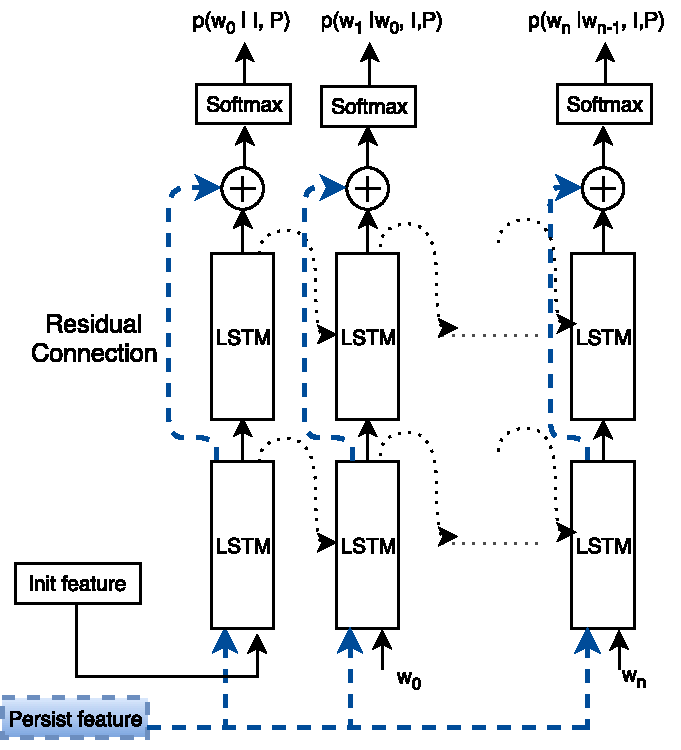
\includegraphics[width=0.7\linewidth]{images/MultilayerResidualLSTM.pdf}
\end{center}
\vspace*{-4mm}
\caption{The proposed language model architecture. The dashed blue lines
        highlight the changes we have proposed over the baseline. 
        Specifically, a two-layer LSTM with residual connections is
        shown.}
\label{fig:proplstmlang}
\end{figure*}

%%===========================================================================%%
\section{Deeper model, residual connections }
\fixme{Upto 1 page: From ACMMM paper}
%% ---------------------------------------------------------------------------
Another extension we experiment with to improve the performance of our language
model is to add depth to the LSTM network used in it.
%%
Here, only the first LSTM layer receives the feature inputs directly and the
higher LSTM layers take their input $x(t)$ from the previous layer in the
network.
%%
The recurrent connections from a network's outputs back to its inputs exist only
within an LSTM layer and not across the layers.
%%
Softmax is applied at the output of the last LSTM layer only.
%%

Our last modification is adding multiple LSTM layers with residual connections
after each layer as proposed in~\cite{He2015} for convolutional neural networks.
%%
These residual connections, shown in Figure~\ref{fig:proplstmlang}, improve the
training convergence speed greatly.
%%
We have also found out that the use of residual connections produces
significantly lower values for both the training cost function and the model
perplexity, as will be detailed in Section~\ref{chapter:results}.

%%===========================================================================%%
\section{Class based Factorization}
\fixme{Upto 1 pages: fresh writing }
Analyzing the baseline language model outputs for errors, one category of
mistakes we often see are where the model misses the fine grain
classification between two closely related objects.
%%
For example we have noticed that a persons gender is often described wrongly.
%%
Similar uncertainty is also seen in telling apart various fruits and vegetables etc.
%%
This happens because these objects often occur in the same contexts, hence
context cannot help differentiate them, and the generator needs to learn really
fine grained classification to get these right.
%%

We hypothesize that this problem arises due to the fact that the language model
essentially needs to do a N way classification at every time-step, where N is
the size of the vocabulary.
%%
When the size of the vocabulary is large, e.g. on COCO dataset the vocabulary
contains 8790 words, this is a hard classification problem.
%%
Additional complexity arises because the errors made in this N-way
classification at any time-step affects all future predictions made during the
generation of that caption.

One idea to address this issue is to split the N-way classification into two
smaller hierarchical classification problems.
%%
To do this, first, the language model vocabulary is split into $K$ classes and
each word in the vocabulary is assigned to one class. 
%%
Now, we can factorize the conditional probability of a word given the context
into two parts as follows:
\begin{equation}
  \label{eq:class} 
  P(w_t | I,P, W^{t-1}) = P(c_t| I,P, W^{t-1})*P(w_t | c_t, I,P,W^{t-1})
\end{equation}
\noindent where $c_t$ is the class of word $w_t$ and $W^{t-1}$ is sequence of words
seen upto time $t-1$, $w_0\cdots w_{t-1}$.

This allows us to split the N-way softmax in the LSTM language model into two
parts, a $N_c$-way softmax to predict the correct class and a $N_{wc}$-way
softmax to predict the correct word within this class.
%%
Here $N_{wc}$ is the number of words within a class.
%%
This hierarchy allows LSTM to learn separate decoders for each class allowing it to
possibly learn fine grained classification.
%%
The hierarchical structure is also more amenable to adding new words to the vocabulary.
%%
Adding a new word to a specific class already transfers the knowledge the model
has about the class to the word, and the model only needs to learn the
distribution of the word within the class.

\subsection{Clustering words into classes}
The first step in implementing the hierarchical structure in the decoder is to
cluster words into different classes.
%%
There are many approaches to do this clustering in the literature.
%%
First category of methods use knowledge bases like Wordnet to find similar words
and group them together.
%%
Second category of methods are completely data driven and use just the training
data statistics to build these clusters.
%%
Here we will look at two different methods relying solely on the coco training
data to cluster words into classes.

\subsubsection{Brown Clustering}
A popular data driven clustering algorithm is \emph{Brown clustering} proposed
in~\cite{BrownClust}
%%
This is a hierarchical clustering algorithm which produces a hierarchical tree
like clusters of all the words in the vocabulary.
%%
First all the words in the vocabulary are considered as individual leaves in a
tree. 
%%
Then at each step two words or classes whose grouping would reduce the clustering
cost function the most are combined into a single class.
%%
The cost function is simply the perplexity assigned by a class based bi-gram
model to the training corpus, which in our case is all the reference captions in
the training set.
%%
Thus this cost function of any given clustering mapping, C, can be written as,
\begin{equation}
  \label{eq:brown} 
        Quality(C) = \frac{1}{n} log \prod_{i=1}^{n} P(C(w_i)|C(w_{i-1})) P(w|C(w_i))
\end{equation}
\noindent where C, is the mapping which assigns words $w$ to their class $C(w)$

The process is terminated once number of leaf nodes have been reduced to the
desired number of clusters. 
%%
Although this process leads to hierarchical clusters, we ignore the hierarchy
and take all the classes in the final clustering output as independent classes
in our language model 
\subsubsection{K-means Clustering}

K-means is a simple yet very effective clustering algorithm which can be used to
cluster numerical data.
%%
The algorithm tries to partition the input data vectors into $k$ clusters such
that each data point belongs to the cluster whose mean vector is closest to it.
%%
Usually, euclidean distance is used to measure distance between data points.
%%
But we cannot directly use this to cluster words as we cannot measure easily the
distance between words.

Instead, we can make use of the word-embeddings which are learnt in our language
model, to represent words as vectors in d-dimensional space.
%%
With this we can measure distance between words and thus utilize K-means
algorithm to cluster words into $K$ classes.
%%
In our experiments, we use the word embeddings learnt in our best language model to
represent the words and run K-means clustering on these word vectors.
%%
Once $K$ cluster centers are obtained, each word is assigned to its closest center
and this partitioning is used in the language model.

\subsection{Factorizing LSTM decoder output}
In order to implement the hierarchical in our LSTM language model, we need to
split the decoder matrix, $W_d$ into a set of $K+1$ smaller matrices.
%%
This set contains one $W_{d\_cls}$  matrix of the size $\text{LSTM hidden size}
\times k$
which is used to compute class probability.
%%
It also has K class specific matrices ${W_{d}^{1},W_{d}^{2}\cdots W_{d}^{K}}$,
each of size $\text{LSTM hidden size}\times |c^k|$, where $|c^k|$ is the size of class
$c_k$.
%%
Thus computation done to predict the word at time-step $t$ has two stages, first
to predict the right class of the word and then using the class specific decoder
matrix to predict the word within the class.
\begin{align}
        \label{eq:classLStmdecoder}
        P(c_{t}^{k}| I,P, W^{t-1}) &= \text{softmax}(W_{d\_cls} y(t)) \\
        c_t &= argmax_k\left(P(c_{t}^k| I,P, w^{t-1})\right) \\
        P(w_t | I,P, w^{t-1}) &= P(c_t| I,P, w^{t-1}) \cdot \text{softmax}(W_{d}^{c_t} y(t))
\end{align}

Although, in theory this should be faster since we are doing two much smaller
matrix multiplication instead of one large one, due to bottlenecks in our
implementation, this hierarchical decoder as slightly slower, than the single
stage decoder.
%%
This was mainly due to the GPU library restriction that required all class
specific decoder matrices to be of the same size, resulting in lot of wasted
computation.
%%===========================================================================%%
\section{Bi-Directional LSTMs ????}
\fixme{Not sure yet: fresh writing }
%%===========================================================================%%
\section{Ensembling Techniques}
%%----------------------------------%%
Using the many different image features and LSTM language model architectures we
have discussed before, we can train a set of different language models.
%%
When examining the pool of captions generated by such models for a set of
images, we have found out that different models tend to generate the best
captions for different images.
%%
If we could evaluate the suitability of a given caption for a given image, we
could possibly pick out the best candidate from the pool and achieve better
results than with any single model.
%%
Thus in this section we will examine two methods of evaluating the suitability
of a caption to the input image/video and thus effectively ensembling multiple
language models.
%%

Concretely, given an input image/video, $V$, and a set of $p$ candidate
captions, $C_p = \left\{S_1,S_2,\cdots S_p \right\}$, generated by $m$ language
models, $LM = \left\{lm_1,lm_2,\cdots lm_m \right\}$, we wish to find the
evaluation function $E(S|V)$, such that $\text{argmax}_{S_i} E(S_i|V)$ is the
most suitable caption for $V$ in the set $C_p$.

Note that, this is different from using evaluation metrics to evaluate a
captioning system, as here we are evaluating the candidate caption without using
reference captions.
%%
First method relies on the caption generating language models themselves to
evaluate candidate captions, while the second method involves training a
separate evaluator model to measure the similarity between the candidate caption
and the input.
%%
We will examine them in detail in the following subsections.

%%----------------------------------%%
\subsection{Combining Multiple models using Mutual Evaluation}
\fixme{1 or 2 paragraphs: fresh writing }

In this technique, we utilize the same language models which were trained to generate
the captions, to also evaluate the captions.
%%
This is based on the observation that the LSTM language model generates the
caption by recursively computing the probability distribution of the next word
and then sampling from this distribution.
%%
Thus the model also computes the conditional probability of the caption, $S$,
given the input image/video, $V$.
%%
This probability, $P(S|I)$, can be used as a measure of the goodness of the
caption w.r.t the input, and thus used to rank the candidate captions.
%%
Note that this probability is also the basis of the cost function used in the
training as described in section~\ref{subsec:basiclstmodel}

But, the probability distributions the generative language models learn tend to
be biased towards the candidates sampled from their own distributions.
%%
In order to remove this bias, we could get the candidate evaluated by not only
the model which generated it, but also by all the other models in the ensemble.
%%
Thus we get $m$ scores per caption, which is averaged to get the evaluation
function:
\begin{equation}
  \label{eq:cmme} 
  E_{\text{CMME}}(S|V) = \frac{1}{m}\sum_{i=1}^{m} P_{lm_i}(S | V)
\end{equation}
\noindent where $P_{lm_i}$ is the probability distribution learned by model
$lm_i$

Since in this method models are evaluating each others sentences, we refer to it
as \emph{Combining Multiple Models with Mutual Evaluation}~(CMME).
%%
This method is also similar to the peer-review model used in academic
publishing, where researchers with expertise in related fields evaluate each
others work.
%%
It works best when all the models in the ensemble are equally competitive, with
expertise in slightly different sub-domains of the dataset.

%%----------------------------------%%
\subsection{CNN Evaluator}
\fixme{1 page: from report}
The language models we used in CMME for evaluation of a candidate caption are
trained generatively.
%%
Thus they need to learn to model both the semantic and syntactic structures of a
sentence and their relation to the input image.
%%
But, in our experiments, we have noticed that these language models are very
effective at learning to syntactic structures of sentences, and grammatical
mistakes are rare in the generated captions.
%%
Most of the errors in the generated captions are of semantic nature, wherein the
models tend to get the objects or relations between objects wrong.
%%
This could be because similar syntactic structure repeat across large portions
of the reference captions in the dataset, but similar semantic relations are
found only in small parts of the dataset.

This means, the evaluator function we use should mainly focus on evaluating the
semantic correctness of the candidate captions, and not worry about
nitty-gritties of syntactic correctness. 
%%
Thus a generatively trained model, like in case of CMME, will be suboptimal at
this task and discriminative training would more suitable. 
%%

We attempt to implement this idea by training a new model whose task
is to pick out the best candidate from the candidate set, given an
input image or video.
%%
We refer to this as an evaluator network.
%%
The model takes as input one visual feature vector and an input sentence and
computes a similarity metric between the sentence and the image. 
%%
Thus the model is composed of a convolutional network to encode the sentences
into a sentence embedding, and a projection matrix which projects the visual
feature into the same space as the sentence embedding.
%%
Then a cosine similarity measure is used to evaluate the similarity between the
sentence embedding vector and the projected visual feature vector. 
%%

The convolutional network we use to encode sentences is based on the
paper~\cite{kim:2014:CNNsent}, where it is used for sentence sentiment
prediction.
%%
Figure~\ref{fig:CNNEval} shows the block diagram of our CNN-based evaluator.  
%%
Here, the input sentence is represented as a sequence of word vectors, which are
either statically initialized with some standard word vector encodings, such as
GloVe~\cite{pennington2014glove} or word2vec~\cite{mikolov2013distributed}, or
learned during the training phase.
%%
These word vectors are fed into a convolutional neural network which computes an
encoding of the sentence.

%%To compute the similarity between the image and the sentence encoding, the image
%%feature vector is first projected into same representation space using a
%%projection matrix.
%%%%
%%The similarity is then computed between the projected image vector and the
%%sentence encoding to give a match score between the input image and the
%%candidate sentence.

\begin{figure*}[t] 
  \centering
  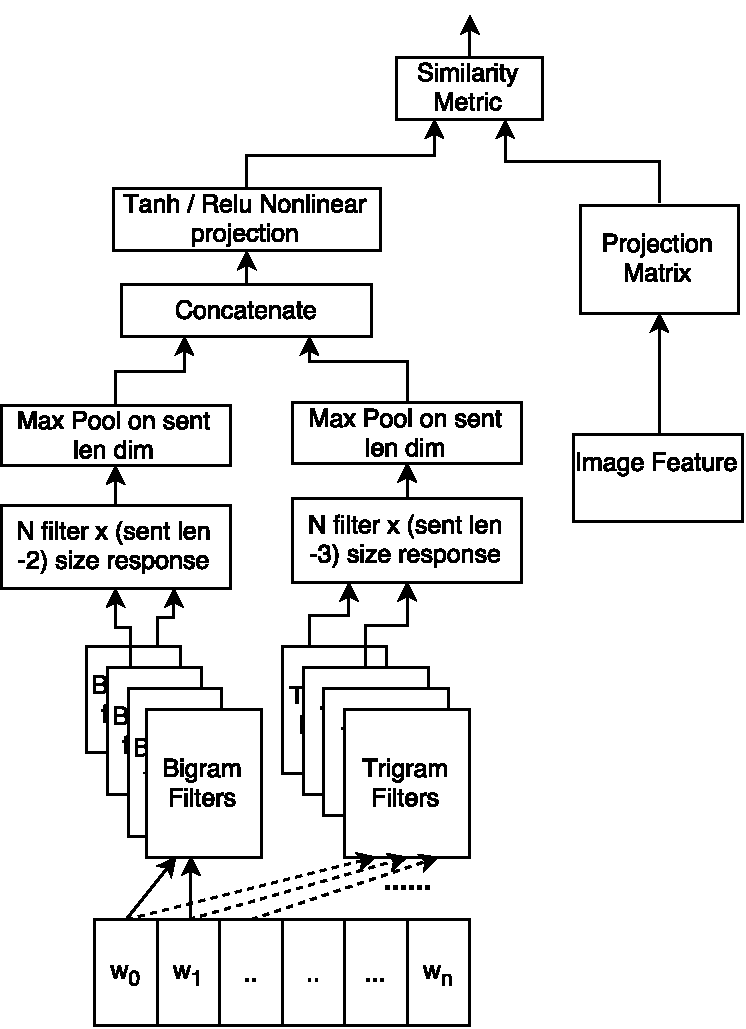
\includegraphics[width=0.6\textwidth]{./images/CnnEval.pdf} 
  \caption{CNN based evaluator network to compute the similarity between 
    an image and a caption.}
  \label{fig:CNNEval} 
\end{figure*}

% Convolutional network on sentences

The first layer in the CNN consists of convolutional filters of different sizes.  
%%
All the filters operate over entire word vectors, but vary in the number of
words they cover, i.e., each filter is of the size $N_{\text{gram}} \times
N_{\text{word vec dim}}$. 
%%
We can thus have filters operating over bigrams, trigrams, etc.
%%
Specifically, our model has filters with bigrams, trigrams, 4-grams and 5-grams. 
%%
Additionally, we use many filters of any given size and so the total number of
filters in the models can be written as $N_{\text{filt}} \cdot N_{\text{filt
type}}$.

The filter outputs are max-pooled, which reduces the filter response over entire
sentence into a single scalar, i.e., its maximum response. 
%%
We can therefore think of each filter as looking for a specific n-gram,
disregarding its location within the sentence.
%%
These pooled outputs are concatenated and then projected to the desired vector
size to produce the final sentence encoding.

%% --------------------------------------

\subsubsection{Training the Evaluator Network}

The evaluator network is trained to assign a high score for the correct or the
best caption and a lower scores for other captions.
%%
This is done by letting the network, for each training set image or video $V$,
to score its ground truth caption, $S^+$, and $k$ negative samples, $S_i^-,
i=1,\ldots,k$, drawn randomly from the ground truth captions of other media in
the training dataset.
%%
Now the training cost function $C$ is devised to maximize the score for the
positive sample and to minimize it for the negative samples. 
%%
This is achieved by applying a softmax on the scores of this batch (one positive
and $k$ negative samples) and maximize the softmax score
of the positive sample:
%%
\begin{align}
  \label{eq:cnnprob} 
  P(S^+|S^-,I) &= \frac{\exp(-f(S^+,I))}{\exp(-f(S^+,I)) +
           \sum\limits_i^k{\exp(-f(S_i^- ,I))}} \\
  C &= -\log P(S^+|S^-,I) \;.
\end{align}
%%
Equation~(\ref{eq:cnnprob}) shows this computation with $f(S,I)$ representing
the similarity metric between the sentence candidate $S$ and media $V$.
%%
In our current method, we use the cosine similarity between the two vectors for
the purpose of $f(S,I)$.

%% --------------------------------------

\subsubsection{Utilizing the Evaluator Network}

Once trained, we can then use the evaluator network to compute the similarity
between each candidate in the pool of captions and the visual feature vector. 
%%
The candidate with the highest similarity is chosen as the output caption from
the ensemble for the input media.

%% ===========================================================================
%%----------------------------------%%
\subsection{BiLstm Evaluator}
\fixme{0.5 page: fresh writing}
